\hypertarget{Convenience_8c}{
\section{Convenience.c File Reference}
\label{Convenience_8c}\index{Convenience.c@{Convenience.c}}
}
{\tt \#include \char`\"{}party.h\char`\"{}}\par


Include dependency graph for Convenience.c:\begin{figure}[H]
\begin{center}
\leavevmode
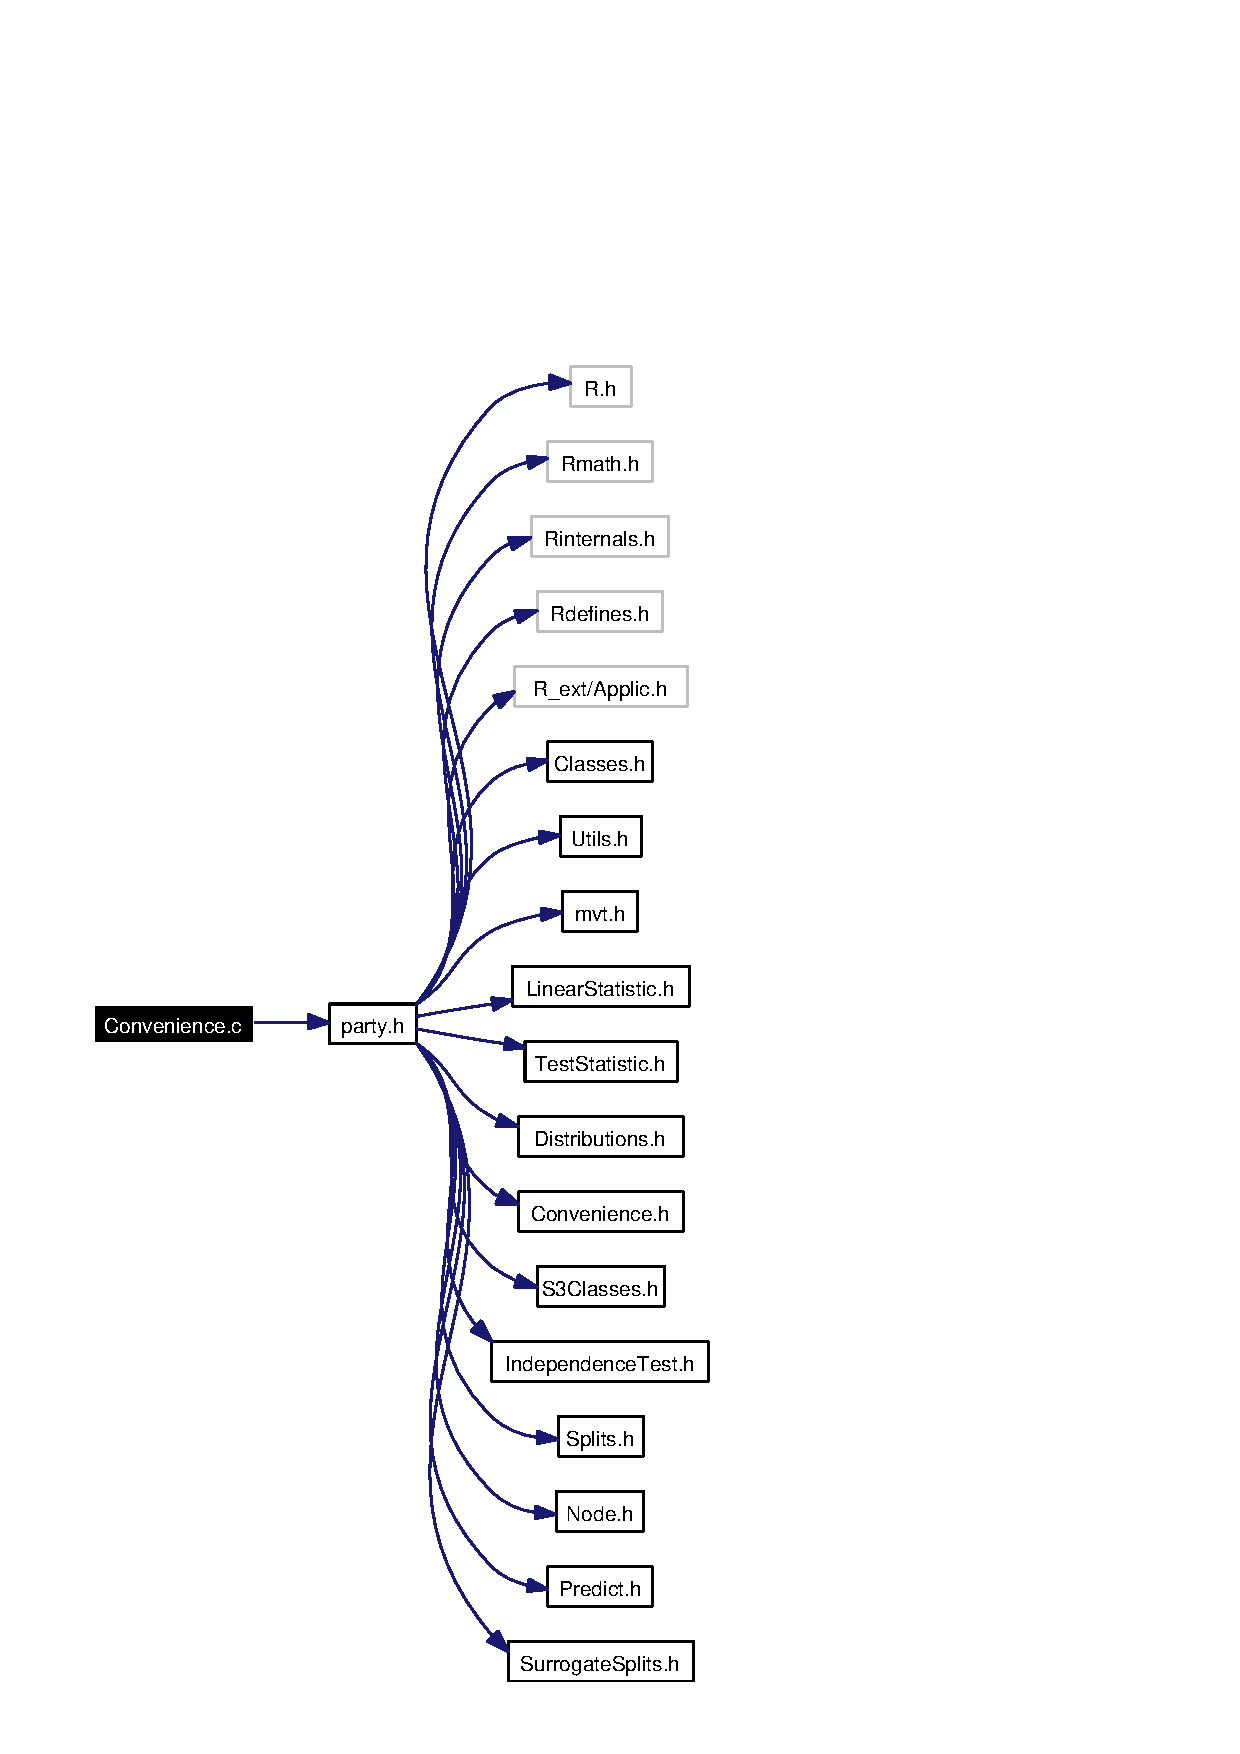
\includegraphics[width=173pt]{Convenience_8c__incl}
\end{center}
\end{figure}
\subsection*{Functions}
\begin{CompactItemize}
\item 
void \hyperlink{Convenience_8c_a0}{C\_\-Lin\-Stat\-Exp\-Cov} (const double $\ast$x, const int p, const double $\ast$y, const int q, const double $\ast$weights, const int n, const int cexpcovinf, SEXP expcovinf, SEXP ans)
\item 
void \hyperlink{Convenience_8c_a1}{C\_\-Lin\-Stat\-Exp\-Cov\-MPinv} (SEXP linexpcov, double tol)
\item 
void \hyperlink{Convenience_8c_a2}{C\_\-MLinear\-Statistic} (SEXP linexpcov, SEXP Score\-Matrix, SEXP ans)
\item 
double \hyperlink{Convenience_8c_a3}{C\_\-Test\-Statistic} (const SEXP linexpcov, const int type, const double tol)
\item 
double \hyperlink{Convenience_8c_a4}{C\_\-Conditional\-Pvalue} (const double tstat, SEXP linexpcov, const int type, double tol, int $\ast$maxpts, double $\ast$releps, double $\ast$abseps)
\item 
SEXP \hyperlink{Convenience_8c_a5}{R\_\-get\_\-response} (SEXP learnsample)
\item 
void \hyperlink{Convenience_8c_a6}{R\_\-set\_\-response} (SEXP learnsample, SEXP y)
\end{CompactItemize}


\subsection{Detailed Description}
Some convenience functions

\begin{Desc}
\item[Author:]\begin{Desc}
\item[Author]hothorn \end{Desc}
\end{Desc}
\begin{Desc}
\item[Date:]\begin{Desc}
\item[Date]2005-08-31 09:27:04 +0200 (Wed, 31 Aug 2005) \end{Desc}
\end{Desc}


Definition in file \hyperlink{Convenience_8c-source}{Convenience.c}.

\subsection{Function Documentation}
\hypertarget{Convenience_8c_a4}{
\index{Convenience.c@{Convenience.c}!C_ConditionalPvalue@{C\_\-ConditionalPvalue}}
\index{C_ConditionalPvalue@{C\_\-ConditionalPvalue}!Convenience.c@{Convenience.c}}
\subsubsection[C\_\-ConditionalPvalue]{\setlength{\rightskip}{0pt plus 5cm}double C\_\-Conditional\-Pvalue (const double {\em tstat}, SEXP {\em linexpcov}, const int {\em type}, double {\em tol}, int $\ast$ {\em maxpts}, double $\ast$ {\em releps}, double $\ast$ {\em abseps})}}
\label{Convenience_8c_a4}


Compute asymptotic conditional P-value \begin{Desc}
\item[Parameters:]
\begin{description}
\item[{\em tstat}]test statistic \item[{\em linexpcov}]an object of class `Lin\-Stat\-Expect\-Covar' \item[{\em type}]integer, 1 (maxabs) or 2 (quadform) \item[{\em tol}]tolerance \item[{\em maxpts}]argument to C\_\-maxabs\-Conditional\-Pvalue \item[{\em releps}]argument to C\_\-maxabs\-Conditional\-Pvalue \item[{\em abseps}]argument to C\_\-maxabs\-Conditional\-Pvalue\end{description}
\end{Desc}


Definition at line 131 of file Convenience.c.

References C\_\-maxabs\-Conditional\-Pvalue(), C\_\-quadform\-Conditional\-Pvalue(), get\_\-dimension(), MAXABS, PL2\_\-covariance\-Sym, PL2\_\-rank\-Sym, and QUADFORM.

Referenced by C\_\-Teststat\-Pvalue().

Here is the call graph for this function:\begin{figure}[H]
\begin{center}
\leavevmode
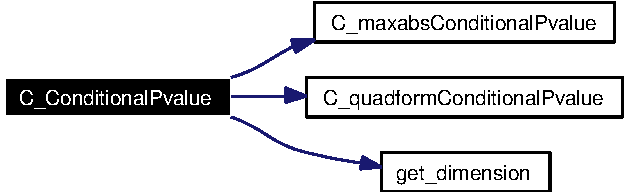
\includegraphics[width=167pt]{Convenience_8c_a4_cgraph}
\end{center}
\end{figure}
\hypertarget{Convenience_8c_a0}{
\index{Convenience.c@{Convenience.c}!C_LinStatExpCov@{C\_\-LinStatExpCov}}
\index{C_LinStatExpCov@{C\_\-LinStatExpCov}!Convenience.c@{Convenience.c}}
\subsubsection[C\_\-LinStatExpCov]{\setlength{\rightskip}{0pt plus 5cm}void C\_\-Lin\-Stat\-Exp\-Cov (const double $\ast$ {\em x}, const int {\em p}, const double $\ast$ {\em y}, const int {\em q}, const double $\ast$ {\em weights}, const int {\em n}, const int {\em cexpcovinf}, SEXP {\em expcovinf}, SEXP {\em ans})}}
\label{Convenience_8c_a0}


Linear statistic of x, y, and weights and its conditional expectation and covariance \par
 \begin{Desc}
\item[Parameters:]
\begin{description}
\item[{\em x}]values of the transformation \item[{\em p}]dimension of the transformation \item[{\em y}]values of the influence function \item[{\em q}]dimension of the influence function \item[{\em weights}]case weights \item[{\em n}]number of observations \item[{\em cexpcovinf}]logical: recompute exp and cov of the influence fct \item[{\em expcovinf}]an object of class `Expect\-Covar\-Influence' \item[{\em ans}]return value; an object of class `Lin\-Stat\-Expect\-Covar'\end{description}
\end{Desc}


Definition at line 26 of file Convenience.c.

References C\_\-Expect\-Covar\-Influence(), C\_\-Expect\-Covar\-Linear\-Statistic(), C\_\-Linear\-Statistic(), and PL2\_\-linearstatistic\-Sym.

Referenced by C\_\-Global\-Test(), C\_\-Independence\-Test(), and R\_\-splitcategorical().

Here is the call graph for this function:\begin{figure}[H]
\begin{center}
\leavevmode
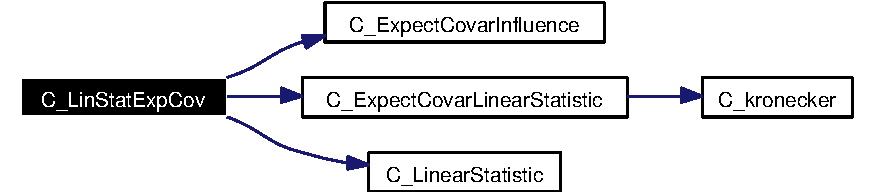
\includegraphics[width=214pt]{Convenience_8c_a0_cgraph}
\end{center}
\end{figure}
\hypertarget{Convenience_8c_a1}{
\index{Convenience.c@{Convenience.c}!C_LinStatExpCovMPinv@{C\_\-LinStatExpCovMPinv}}
\index{C_LinStatExpCovMPinv@{C\_\-LinStatExpCovMPinv}!Convenience.c@{Convenience.c}}
\subsubsection[C\_\-LinStatExpCovMPinv]{\setlength{\rightskip}{0pt plus 5cm}void C\_\-Lin\-Stat\-Exp\-Cov\-MPinv (SEXP {\em linexpcov}, double {\em tol})}}
\label{Convenience_8c_a1}


Moore-Penrose inverse of the covariance matrix \par
 \begin{Desc}
\item[Parameters:]
\begin{description}
\item[{\em linexpcov}]an object of class `Lin\-Stat\-Expect\-Covar\-MPinv' \item[{\em tol}]tolerance\end{description}
\end{Desc}


Definition at line 46 of file Convenience.c.

References C\_\-MPinv(), PL2\_\-covariance\-Sym, and PL2\_\-svdmem\-Sym.

Referenced by C\_\-Global\-Test(), and C\_\-Independence\-Test().

Here is the call graph for this function:\begin{figure}[H]
\begin{center}
\leavevmode
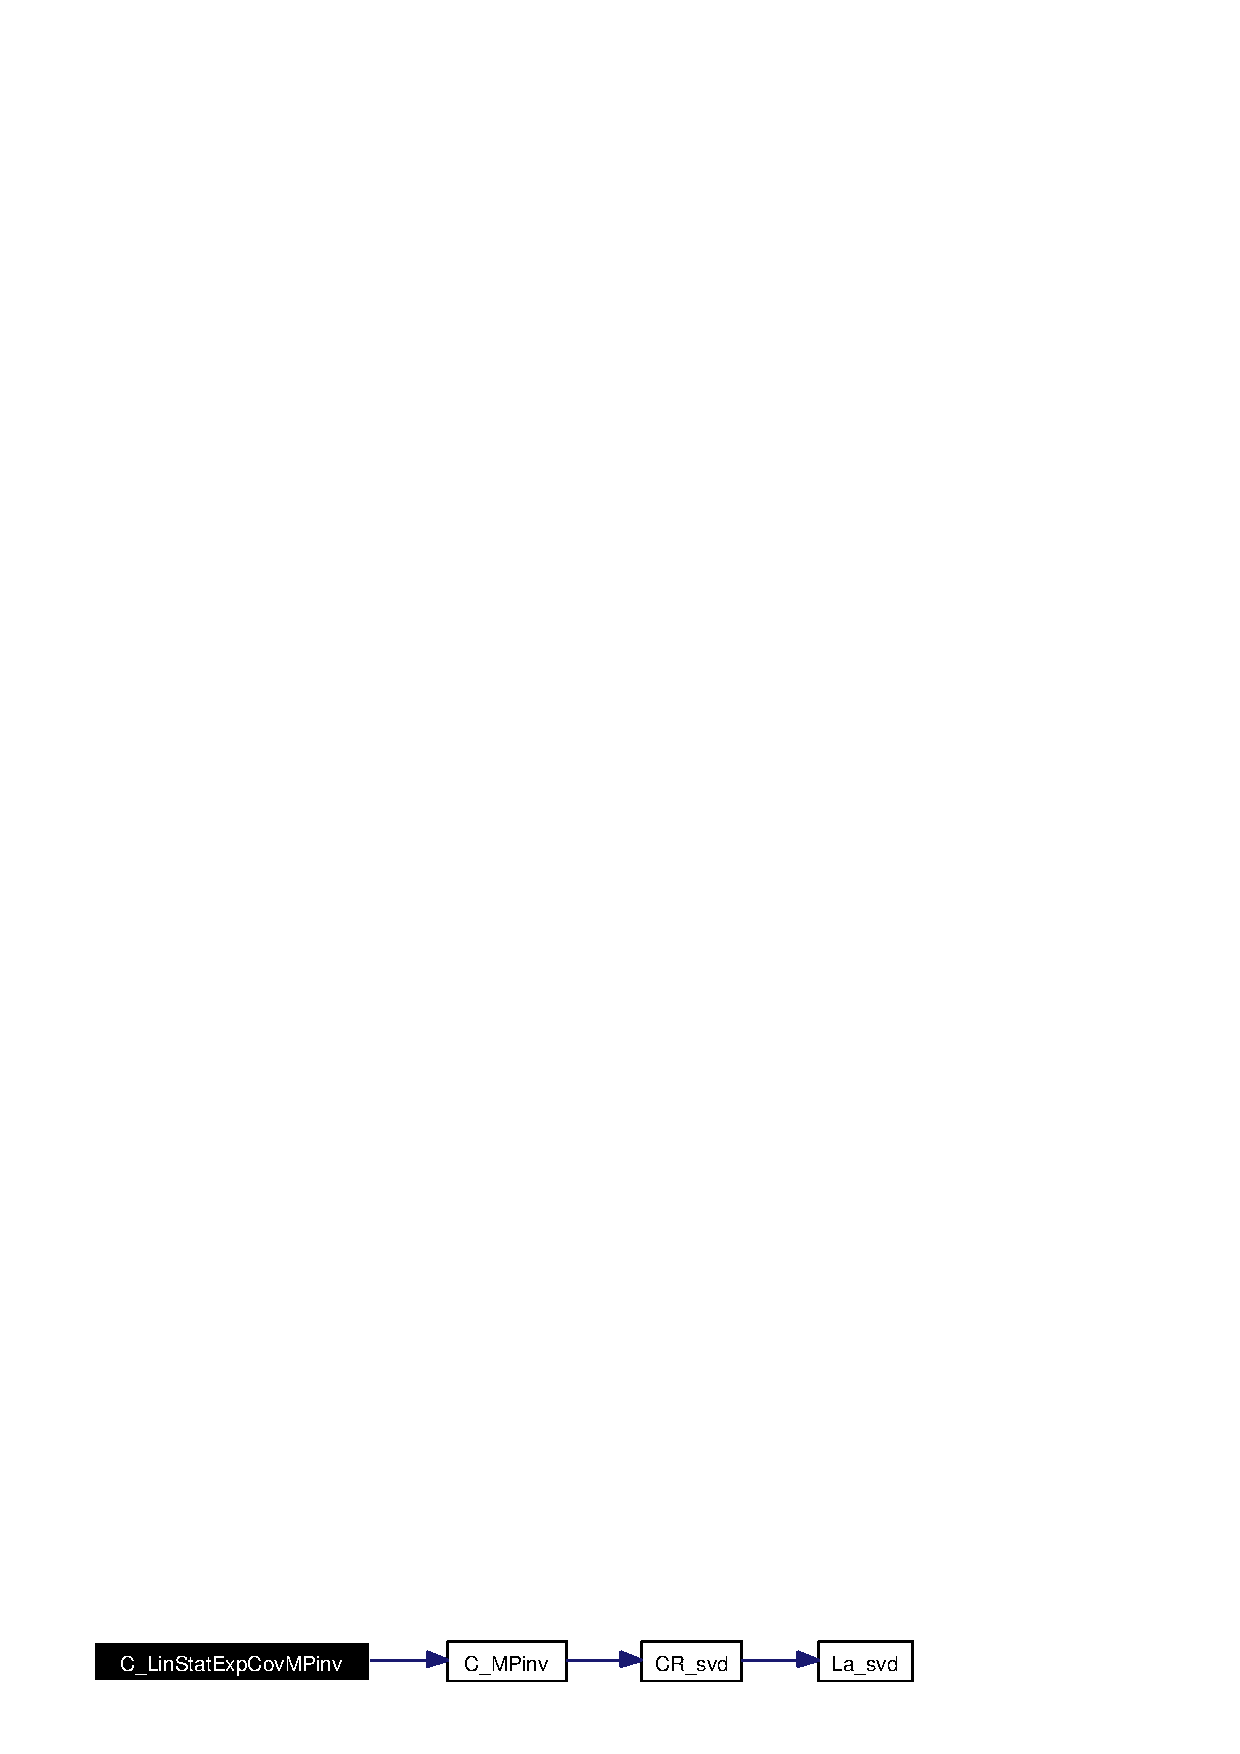
\includegraphics[width=214pt]{Convenience_8c_a1_cgraph}
\end{center}
\end{figure}
\hypertarget{Convenience_8c_a2}{
\index{Convenience.c@{Convenience.c}!C_MLinearStatistic@{C\_\-MLinearStatistic}}
\index{C_MLinearStatistic@{C\_\-MLinearStatistic}!Convenience.c@{Convenience.c}}
\subsubsection[C\_\-MLinearStatistic]{\setlength{\rightskip}{0pt plus 5cm}void C\_\-MLinear\-Statistic (SEXP {\em linexpcov}, SEXP {\em Score\-Matrix}, SEXP {\em ans})}}
\label{Convenience_8c_a2}


Linear combination of a linear statistic, expectation and covariance \begin{Desc}
\item[Parameters:]
\begin{description}
\item[{\em linexpcov}]an object of class `Lin\-Stat\-Expect\-Covar' \item[{\em Score\-Matrix}]matrix of coefficients \item[{\em ans}]return value; an object of class `Lin\-Stat\-Expect\-Covar'\end{description}
\end{Desc}


Definition at line 59 of file Convenience.c.

References C\_\-matprod(), C\_\-matprod\-T(), get\_\-dimension(), ncol(), nrow(), PL2\_\-covariance\-Sym, PL2\_\-expectation\-Sym, and PL2\_\-linearstatistic\-Sym.

Referenced by C\_\-Global\-Test(), C\_\-Independence\-Test(), and C\_\-Monte\-Carlo().

Here is the call graph for this function:\begin{figure}[H]
\begin{center}
\leavevmode
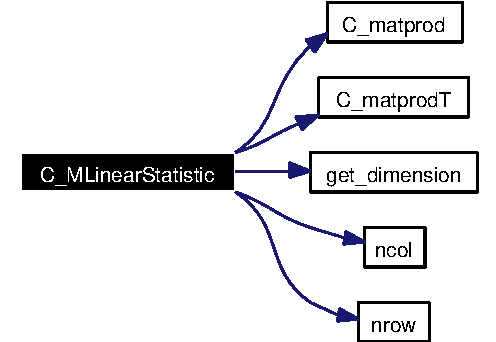
\includegraphics[width=128pt]{Convenience_8c_a2_cgraph}
\end{center}
\end{figure}
\hypertarget{Convenience_8c_a3}{
\index{Convenience.c@{Convenience.c}!C_TestStatistic@{C\_\-TestStatistic}}
\index{C_TestStatistic@{C\_\-TestStatistic}!Convenience.c@{Convenience.c}}
\subsubsection[C\_\-TestStatistic]{\setlength{\rightskip}{0pt plus 5cm}double C\_\-Test\-Statistic (const SEXP {\em linexpcov}, const int {\em type}, const double {\em tol})}}
\label{Convenience_8c_a3}


Compute test statistic \begin{Desc}
\item[Parameters:]
\begin{description}
\item[{\em linexpcov}]an object of class `Lin\-Stat\-Expect\-Covar' \item[{\em type}]integer, 1 (maxabs) or 2 (quadform) \item[{\em tol}]tolerance\end{description}
\end{Desc}


Definition at line 91 of file Convenience.c.

References C\_\-maxabs\-Test\-Statistic(), C\_\-quadform\-Test\-Statistic(), get\_\-dimension(), PL2\_\-covariance\-Sym, PL2\_\-expectation\-Sym, PL2\_\-linearstatistic\-Sym, and PL2\_\-MPinv\-Sym.

Referenced by C\_\-Teststat\-Pvalue().

Here is the call graph for this function:\begin{figure}[H]
\begin{center}
\leavevmode
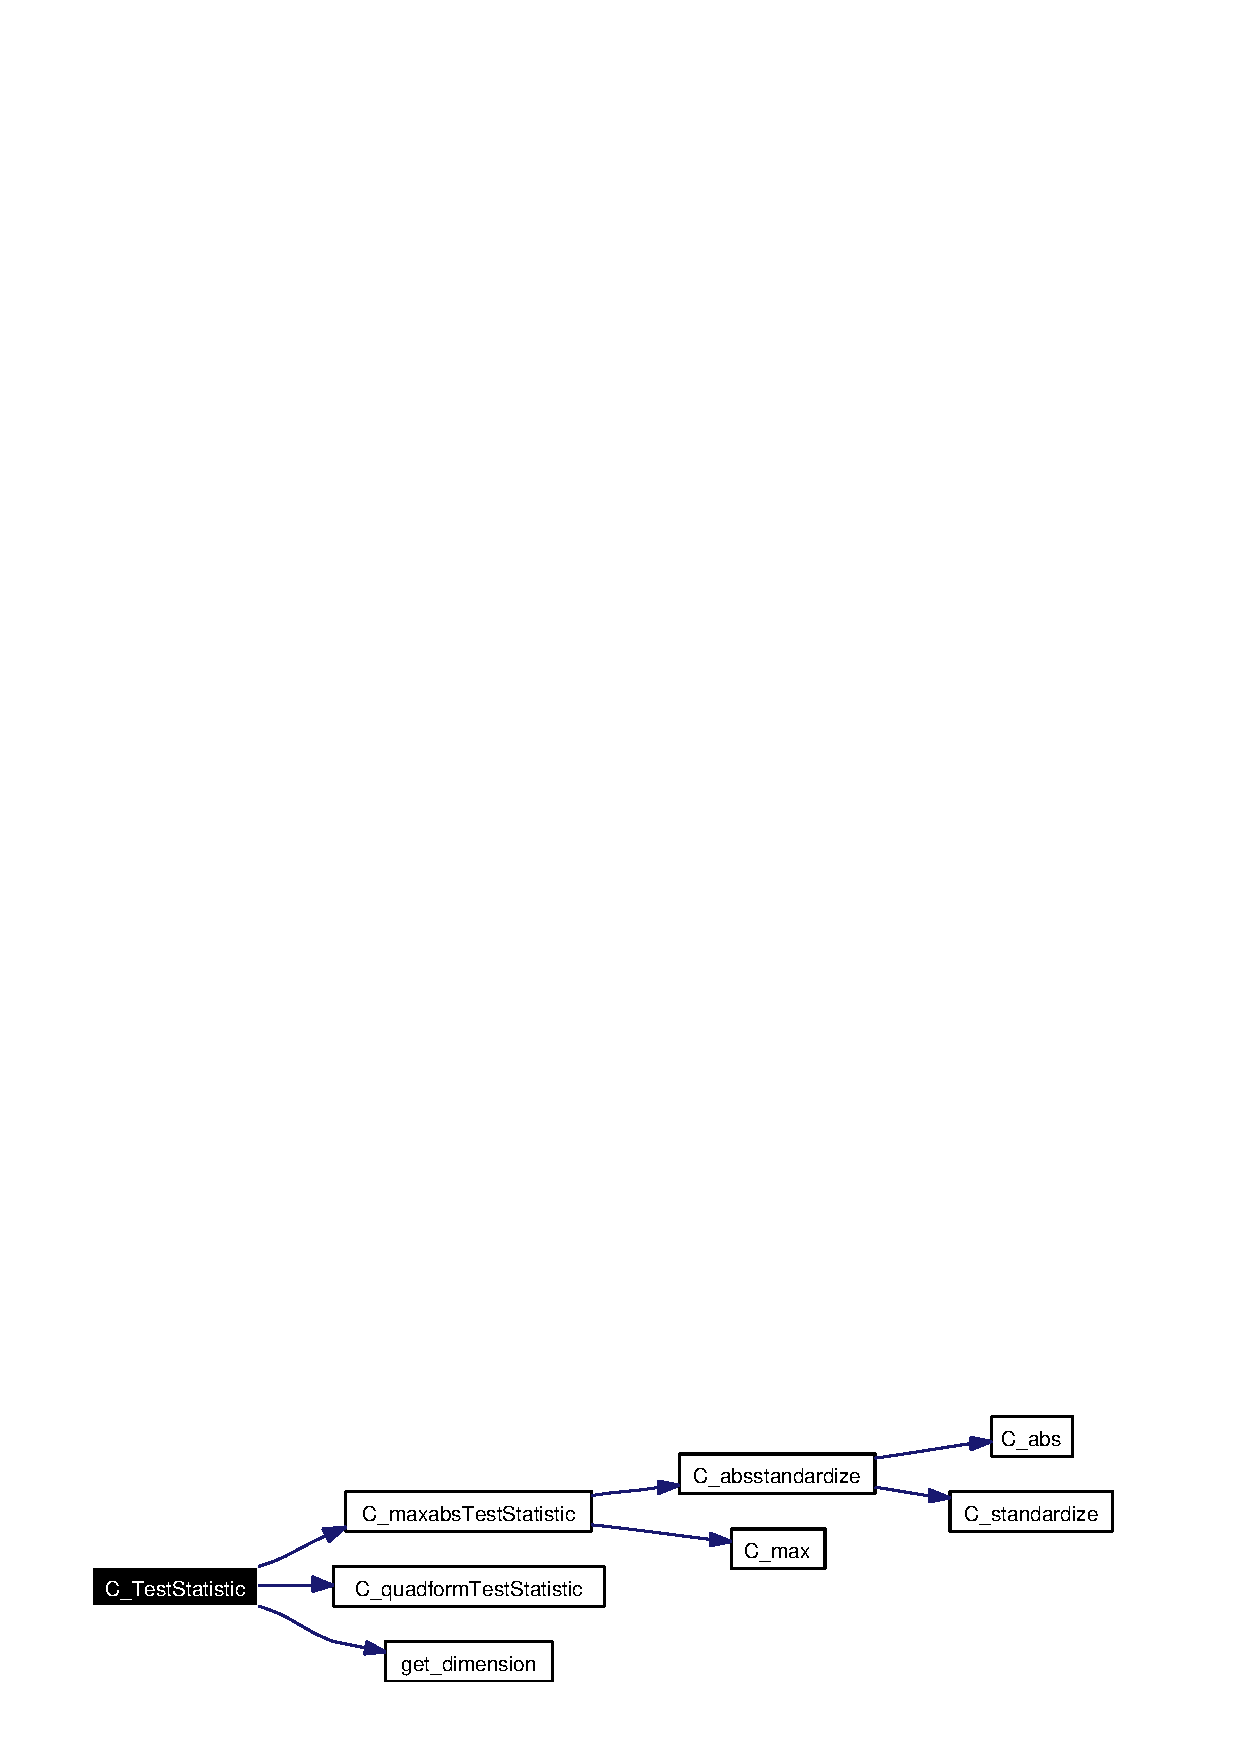
\includegraphics[width=267pt]{Convenience_8c_a3_cgraph}
\end{center}
\end{figure}
\hypertarget{Convenience_8c_a5}{
\index{Convenience.c@{Convenience.c}!R_get_response@{R\_\-get\_\-response}}
\index{R_get_response@{R\_\-get\_\-response}!Convenience.c@{Convenience.c}}
\subsubsection[R\_\-get\_\-response]{\setlength{\rightskip}{0pt plus 5cm}SEXP R\_\-get\_\-response (SEXP {\em learnsample})}}
\label{Convenience_8c_a5}


extract the (first) response variable from a learning sample \begin{Desc}
\item[Parameters:]
\begin{description}
\item[{\em learnsample}]an object of class `Learning\-Sample'\end{description}
\end{Desc}


Definition at line 163 of file Convenience.c.

References PL2\_\-responses\-Sym, and PL2\_\-variables\-Sym.

Referenced by R\_\-set\_\-response().\hypertarget{Convenience_8c_a6}{
\index{Convenience.c@{Convenience.c}!R_set_response@{R\_\-set\_\-response}}
\index{R_set_response@{R\_\-set\_\-response}!Convenience.c@{Convenience.c}}
\subsubsection[R\_\-set\_\-response]{\setlength{\rightskip}{0pt plus 5cm}void R\_\-set\_\-response (SEXP {\em learnsample}, SEXP {\em y})}}
\label{Convenience_8c_a6}


change the values of the response variable in a learning sample \begin{Desc}
\item[Parameters:]
\begin{description}
\item[{\em learnsample}]an object of class `Learning\-Sample' \item[{\em y}]a REAL with new values\end{description}
\end{Desc}


Definition at line 175 of file Convenience.c.

References PL2\_\-jointtransf\-Sym, PL2\_\-responses\-Sym, PL2\_\-transformations\-Sym, PL2\_\-variables\-Sym, and R\_\-get\_\-response().

Here is the call graph for this function:\begin{figure}[H]
\begin{center}
\leavevmode

\includegraphics[width=126pt]{Convenience_8c_a6_cgraph}
\end{center}
\end{figure}
